% !TEX program = pdflatex
\documentclass[journal]{IEEEtran}

% ──────────────────────────────────────────────────────────────────────────────
%  Packages
% ──────────────────────────────────────────────────────────────────────────────
\usepackage[T1]{fontenc}
\usepackage{amsmath,amssymb,amsfonts,amsthm}
\usepackage{algorithmic}
\usepackage[ruled,linesnumbered]{algorithm2e}
\usepackage{tikz}
\usepackage{graphicx}
\usepackage{textcomp}
\usepackage{xcolor}
\usepackage{booktabs}
\usepackage{multirow}
\usepackage{hyperref}
\usepackage{cleveref}
\usepackage{bm}
\usepackage{mathtools}
\usepackage{subcaption}
\usepackage{siunitx}
\usepackage{balance}

% Theorem environments
\newtheorem{theorem}{Theorem}
\newtheorem{lemma}[theorem]{Lemma}
\newtheorem{corollary}[theorem]{Corollary}
\newtheorem{definition}[theorem]{Definition}
\newtheorem{remark}{Remark}
\newtheorem{assumption}{Assumption}
\newtheorem{proposition}{Proposition}

% Notation shortcuts
\newcommand{\Cfree}{\mathcal{C}_{\mathrm{free}}}
\newcommand{\Cspace}{\mathcal{C}}
\newcommand{\IR}{I_{\!R}}
\newcommand{\IE}{I_{\!E}}
\newcommand{\dR}{d_{\!R}}
\newcommand{\SPD}{\mathbb{S}_{++}^{d}}
\newcommand{\muR}{\mu_{\!R}}
\newcommand{\Vol}{\mathrm{Vol}}
\newcommand{\diag}{\mathrm{diag}}
\DeclareMathOperator*{\argmin}{arg\,min}

% IEEE specific
\IEEEoverridecommandlockouts

\begin{document}

% ══════════════════════════════════════════════════════════════════════════════
%  TITLE
% ══════════════════════════════════════════════════════════════════════════════
\title{RIT*: Riemannian Informed Trees for\\Anisotropic Motion Planning}

\author{
  \IEEEauthorblockN{Author~Names~Omitted~for~Review}
  \IEEEauthorblockA{Affiliation Omitted for Review}
}

\markboth{IEEE Robotics and Automation Letters}{Author~et~al.: RIT*: Riemannian Informed Trees}

\maketitle

% ══════════════════════════════════════════════════════════════════════════════
%  ABSTRACT  (~150 words)
% ══════════════════════════════════════════════════════════════════════════════
\begin{abstract}
Asymptotically-optimal sampling-based planners accelerate convergence
by focusing sampling within an informed set, but all existing methods
define this set using Euclidean distance.
When traversal costs are anisotropic---as with joint-inertia weighting
or obstacle-proximity penalties---the Euclidean informed set wastes
samples in regions that cannot contain improving paths.
We present \textbf{RIT*} (Riemannian Informed Trees), which replaces
the Euclidean informed set, neighbourhood ball, and edge cost with
their Riemannian counterparts, yielding a provably smaller sampling
region.
RIT* includes a Collision-Adaptive Riemannian Metric (CARM) module
that learns a cost field online from collision feedback, requiring no
a~priori obstacle model.
Experiments on 2-D through 6-DOF UR10e manipulator environments show
that RIT* reduces path cost by up to 11\% over five baselines in
constrained manipulator planning, while CARM recovers up to 27\%
of the oracle-metric advantage using only a binary collision checker.
\end{abstract}

\begin{IEEEkeywords}
Motion planning, Riemannian geometry, asymptotic optimality,
informed sampling, online metric learning.
\end{IEEEkeywords}

% ══════════════════════════════════════════════════════════════════════════════
%  OVERVIEW FIGURE
% ══════════════════════════════════════════════════════════════════════════════
\begin{figure*}[t]
\centering
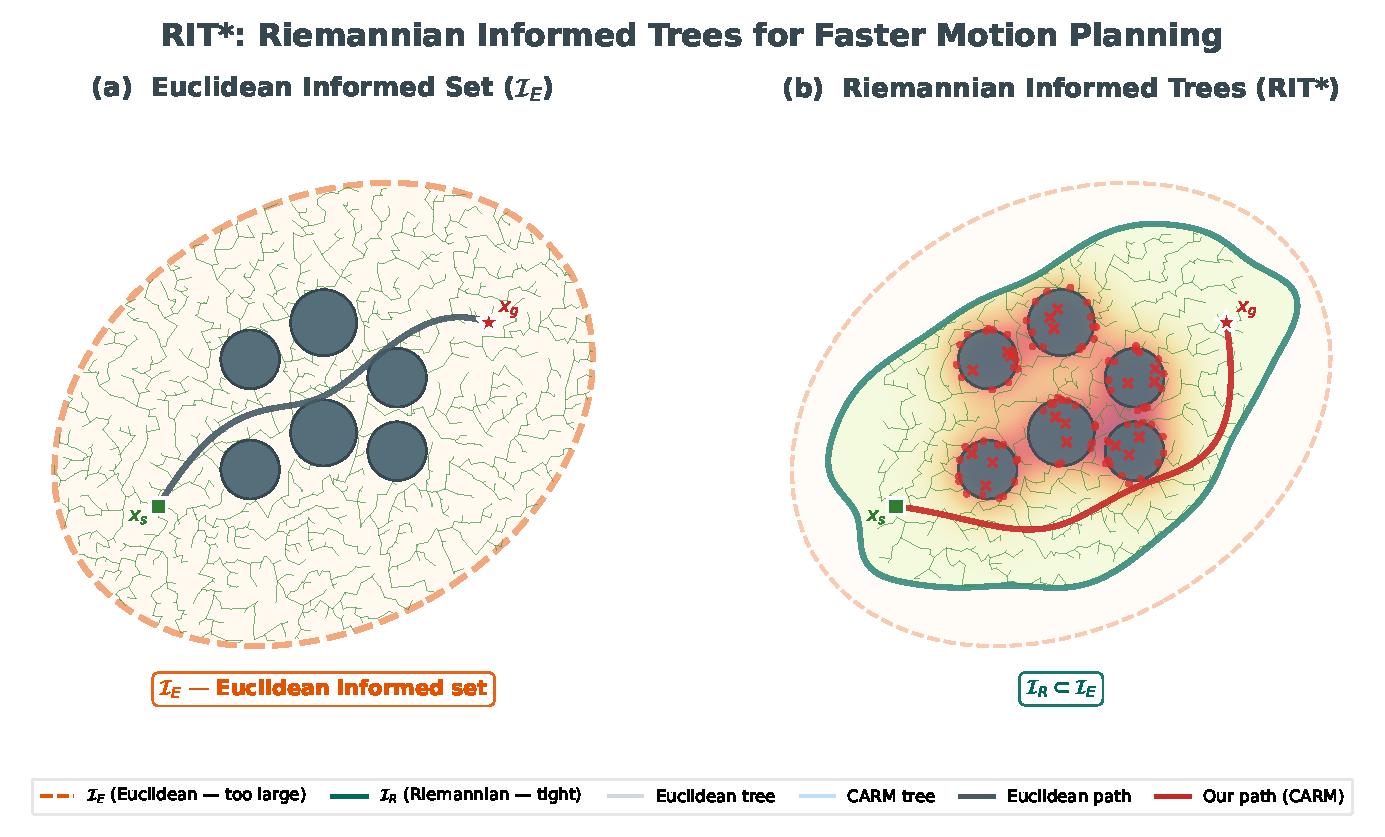
\includegraphics[width=\textwidth]{figures/fig_abstract.pdf}
\caption{Overview of RIT*.
  \textbf{(a)}~Euclidean planners sample uniformly from the
  informed set~$\IE$ (orange ellipse), wasting
  samples in high-cost regions near obstacles.
  \textbf{(b)}~RIT* replaces every Euclidean primitive with its
  Riemannian counterpart: the tighter informed set~$\IR
  \subset \IE$ (teal) eliminates wasted volume; the anisotropic
  neighbourhood ball reaches further along cheap directions;
  a three-level cascade rejects the majority of candidate edges
  before expensive integration; and the CARM module learns a cost
  field online from collision feedback, progressively tightening
  $\IR$.}
\label{fig:abstract}
\end{figure*}


% ══════════════════════════════════════════════════════════════════════════════
%  I. INTRODUCTION
% ══════════════════════════════════════════════════════════════════════════════
\section{Introduction}\label{sec:intro}

%--- Paragraph 1: Motivation ---
Manipulator motion planning requires optimizing paths under
non-Euclidean costs: joint-inertia weighting penalizes motion of
high-inertia joints, obstacle-proximity penalties steer paths away from
collisions, and task-space norms encode end-effector
preferences~\cite{Ratliff2009,Zucker2013}.
A natural framework for such costs is Riemannian geometry, where a
spatially-varying metric tensor~$G(x)$ encodes directional traversal
cost.
Current asymptotically-optimal (AO) planners---from
RRT*~\cite{Karaman2011} through Informed~RRT*~\cite{Gammell2018},
BIT*~\cite{Gammell2020}, AIT*/EIT*~\cite{Strub2022}, to the recent
APT*~\cite{APT2025}---accelerate convergence by sampling within an
\emph{informed set}, but all define this set using Euclidean distance.
When the true cost metric is anisotropic, the Euclidean informed
set~$\IE$ is a strict superset of the cost-relevant region~$\IR$:
for a 6-DOF arm with joint-inertia condition number $\kappa = 12$,
$\IE$ is approximately $3.4\times$ larger than necessary.

%--- Paragraph 2: Gap ---
Two problems remain open.
First, no batch-informed planner uses Riemannian geometry for its
global sampling strategy---informed set, neighbourhood, and edge
cost---as opposed to local steering alone.
Second, no sampling-based planner learns a suitable cost metric online
from planning experience.

%--- Paragraph 3: Contributions ---
\textbf{Contributions.}
We propose \textbf{RIT*} (Riemannian Informed Trees), which addresses
both gaps:
\begin{enumerate}
  \item \textbf{Online metric learning via CARM.}
    The Collision-Adaptive Riemannian Metric (CARM) module is, to our
    knowledge, the first online metric-learning scheme for
    sampling-based planning that requires no a~priori obstacle model,
    no demonstrations, and no auxiliary sensors---only the binary
    collision checker already available to any planner.
    CARM places Gaussian kernels on discovered collision points to
    build an adaptive cost field that inflates traversal cost near
    obstacles, and feeds the learned metric directly into the planning
    loop (\cref{sec:carm}).

  \item \textbf{Riemannian informed planning pipeline.}
    RIT* replaces every Euclidean primitive in the batch-informed
    pipeline with its Riemannian counterpart:
    (i)~a whitening transform maps the Riemannian informed
    set~$\IR$ to a standard prolate hyperspheroid for efficient
    uniform sampling;
    (ii)~neighbours are found within ellipsoidal Riemannian balls
    that reach further along cheap directions;
    (iii)~a three-level cascading edge evaluation scheme filters
    the majority of candidate edges before expensive integration.
    This framework makes CARM's learned metric actionable throughout
    the planning loop.

  \item \textbf{Experimental validation.}
    Multi-trial experiments across eight environments (2-D through
    6-DOF UR10e manipulator) against five baselines show that RIT*
    achieves up to 11\% cost reduction in 6-DOF manipulator
    planning with statistical significance.
    CARM recovers up to 27\% of the oracle-metric advantage
    without any prior cost model.
\end{enumerate}

%--- Paragraphs 4--6: Compressed related work ---
\textbf{Euclidean informed planners.}
Gammell et~al.~\cite{Gammell2018} introduced direct sampling of the
prolate hyperspheroid, which BIT*~\cite{Gammell2020} combines with
batch sampling and lazy edge evaluation.
AIT* and EIT*~\cite{Strub2022} add asymmetric bidirectional search.
APT*~\cite{APT2025} uses Coulomb-force-inspired virtual forces to
prolate the neighbourhood ball and adapts batch size.
FIT*~\cite{FIT2024} adjusts batch size for faster initial convergence.
All define the informed set using Euclidean distance.

\textbf{Riemannian methods in planning.}
CHOMP~\cite{Ratliff2009} and STOMP~\cite{Zucker2013} optimise
trajectories under Riemannian-like costs but are trajectory
optimisers without AO guarantees.
Kyaw and Kelly~\cite{Kyaw2026} propose a Riemannian RRT* using
retractions for local steering; their planner is incremental
(not batch-informed), does not construct an informed set, and does
not learn metrics online.
Bi-AM-RRT*~\cite{Zhang2023biamrrt} uses a diffusion-based metric to
bias nearest-neighbour selection in an incremental framework.
Kim et~al.~\cite{Kim2016} use Riemannian metrics for steering on
constrained manifolds.
None integrate Riemannian geometry into the global informed sampling
strategy of a batch-informed planner.

\textbf{Obstacle-aware Riemannian metrics.}
Klein et~al.~\cite{Klein2023} design region-avoiding metrics using
hand-crafted barrier functions requiring full obstacle geometry.
RMPflow~\cite{Cheng2018rmpflow} composes task-space metrics for
reactive control.
Beik-Mohammadi et~al.~\cite{BeikMohammadi2023} learn Riemannian
manifolds from demonstrations for reactive motion generation.
All require a~priori obstacle geometry or demonstrations---CARM
requires neither.


% ══════════════════════════════════════════════════════════════════════════════
%  II. PROBLEM FORMULATION
% ══════════════════════════════════════════════════════════════════════════════
\section{Problem Formulation}\label{sec:problem}

\subsection*{Configuration Space and Metric}

Let $\Cspace \subseteq \mathbb{R}^d$ be the \emph{configuration space} of a
robotic system with $d$ degrees of freedom.
Each point $x \in \Cspace$ is a configuration vector
(e.g., a vector of joint angles for a $d$-DOF manipulator).
The space is equipped with a \emph{Riemannian metric tensor field}
\[
  G : \Cspace \;\longrightarrow\; \mathbb{S}^d_{++},
\]
where $\mathbb{S}^d_{++}$ denotes the set of $d \!\times\! d$ symmetric
positive-definite matrices.
At every configuration $x$, the matrix $G(x)$ assigns a local inner product
to pairs of velocity vectors: intuitively, directions along which the robot
is heavy or inertially expensive to move are \emph{stretched} by $G(x)$,
so the planner naturally favours moving lighter joints.

\subsection*{Path Cost}

A \emph{path} is a piecewise-smooth curve
$\sigma : [0,1] \to \Cspace$, where $\sigma(0)$ is the start and
$\sigma(1)$ is the goal configuration.
The quantity $\dot{\sigma}(t) \in \mathbb{R}^d$ is the \emph{tangent
vector} (velocity) of the path at parameter value $t$.
The \emph{Riemannian arc-length} of $\sigma$ is
\begin{equation}\label{eq:cost}
  c(\sigma)
  = \int_0^1 \!\underbrace{\sqrt{
      \underbrace{\dot{\sigma}(t)^\top}_{\text{row velocity}}
      \underbrace{G\!\bigl(\sigma(t)\bigr)}_{\substack{\text{local metric}\\\text{matrix}}}
      \underbrace{\dot{\sigma}(t)}_{\text{col.\ velocity}}
    }}_{\text{instantaneous Riemannian speed}}\; dt.
\end{equation}
When $G(x) = I_d$ (the identity matrix) for all $x$, \cref{eq:cost}
reduces to the ordinary Euclidean arc-length $\int_0^1\!\|\dot\sigma(t)\|_2\,dt$.
For a manipulator, setting $G(q) = M(q)$ (the joint-space inertia matrix)
makes $c(\sigma)$ proportional to the total kinetic energy exerted along
the path, penalising motion of high-inertia joints (shoulder, elbow) more
than low-inertia joints (wrist).

\subsection*{Geodesic Distance and Optimal Path}

The \emph{geodesic distance} between two configurations
$x, y \in \Cspace$ is the infimum of $c(\sigma)$ over all paths connecting
them:
\begin{equation}\label{eq:geodesic}
  \dR(x,\,y)
  = \inf_{\sigma\,:\,\sigma(0)=x,\;\sigma(1)=y} c(\sigma).
\end{equation}
When $G = I_d$ this equals the Euclidean distance $\|x - y\|_2$.

Let $\Cfree \subseteq \Cspace$ be the \emph{obstacle-free} subset
of configurations (those for which the robot does not collide with any
obstacle).
Given a \emph{start} configuration $x_s \in \Cfree$ and a
\emph{goal} configuration $x_g \in \Cfree$, the optimal motion-planning
problem is to find
\begin{equation}\label{eq:opt}
  \sigma^*
  = \argmin_{\substack{\sigma\,:\,\sigma(0)=x_s,\;\sigma(1)=x_g \\ \sigma(t)\in\Cfree\;\forall t\in[0,1]}}
    c(\sigma).
\end{equation}
The cost of the optimal path is denoted $c^*$.
A planner is called \emph{asymptotically optimal} (AO) if the cost
$c_n$ of the best solution found after $n$ samples satisfies
$c_n \to c^*$ almost surely as $n \to \infty$.

\subsection*{Informed Sets}

Once a feasible path of cost $c_{\mathrm{best}}$ has been found, any
configuration that cannot lie on a strictly cheaper path can be safely
ignored.
Formally, only configurations $x$ satisfying
$\dR(x_s,x) + \dR(x,x_g) \le c_{\mathrm{best}}$
(i.e., the detour through $x$ cannot beat the current best) need be sampled.
This defines two nested sets.

The \emph{Euclidean informed set}
\begin{equation}\label{eq:IE}
  \IE
  = \bigl\{\, x \in \Cspace
      \;\big|\;
      \underbrace{\|x_s - x\|_2}_{\text{straight-line dist.\ start}\to x}
    + \underbrace{\|x - x_g\|_2}_{\text{straight-line dist.\ }x\to\text{goal}}
    \le c_{\mathrm{best}} \,\bigr\}
\end{equation}
is the standard prolate hyperspheroid used by Informed~RRT* and BIT*.
Because $\|\cdot\|_2$ lower-bounds the true geodesic distance, $\IE$
is a superset of the true admissible region: it may contain many
configurations that cannot actually improve the solution.

The \emph{Riemannian informed set}
\begin{equation}\label{eq:IR}
  \IR
  = \bigl\{\, x \in \Cspace
      \;\big|\;
      \underbrace{\dR(x_s,\, x)}_{\text{Riemannian dist.\ start}\to x}
    + \underbrace{\dR(x,\, x_g)}_{\text{Riemannian dist.\ }x\to\text{goal}}
    \le c_{\mathrm{best}} \,\bigr\}
\end{equation}
uses the true Riemannian geodesic distance, so it is a tighter bound.
Whenever $G(x) \succeq I_d$ (i.e., $G(x) - I_d$ is positive semi-definite),
the Cauchy–Schwarz inequality gives $\dR(x,y) \ge \|x - y\|_2$, which
implies $\IR \subseteq \IE$.
In anisotropic spaces (large condition number $\kappa(G)$), $\IR$ can
be dramatically smaller than $\IE$, concentrating samples where they
matter and accelerating convergence.


% ══════════════════════════════════════════════════════════════════════════════
%  III. METHOD
% ══════════════════════════════════════════════════════════════════════════════
\section{Method}\label{sec:method}

% ─────────────────────────────────────────────
\subsection{Overview}\label{sec:overview}

\begin{figure*}[t]
\centering
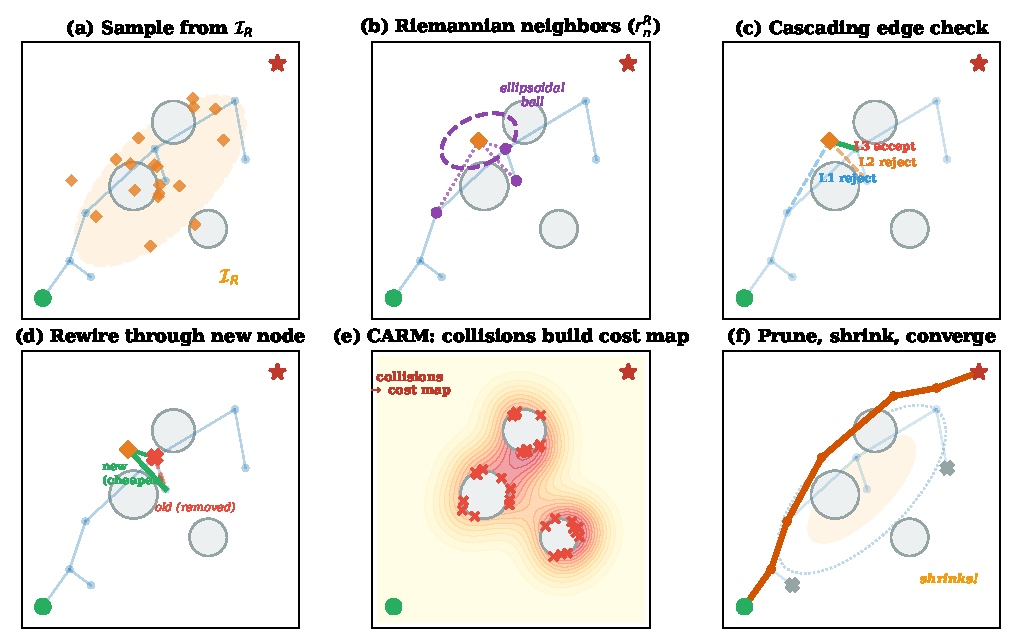
\includegraphics[width=\textwidth]{figures/fig_compact_pipeline.pdf}
\caption{Per-iteration pipeline of RIT*.
  \textbf{(a)}~Samples drawn from the Riemannian informed set~$\IR$.
  \textbf{(b)}~Neighbours identified within ellipsoidal Riemannian
  radius~$r_n^R$.
  \textbf{(c)}~Three-level cascade filters candidate edges
  (L1$\to$L2$\to$L3).
  \textbf{(d)}~Rewiring via cheaper Riemannian connections.
  \textbf{(e)}~CARM collects collision points and rebuilds the
  metric field.
  \textbf{(f)}~Pruning shrinks the informed set as $c_{\mathrm{best}}$
  decreases.}
\label{fig:pipeline}
\end{figure*}

%--- Paragraph 1: BIT* background ---
Our approach builds on BIT* (Batch Informed
Trees)~\cite{Gammell2020}, a state-of-the-art asymptotically-optimal
planner that combines batch sampling with lazy edge evaluation.
BIT* operates in iterations: at each iteration it draws a batch of
$B$ samples from the \emph{Euclidean informed set}~$\IE$---the
prolate hyperspheroid containing all configurations that could lie on
a path shorter than the current best cost~$c_{\mathrm{best}}$.
It then connects each sample to nearby vertices whose Euclidean
distance falls within a shrinking connection radius
$r_n = \gamma\,(\log n / n)^{1/d}$, evaluates candidate parent edges
in order of estimated cost-to-come, rewires the tree when cheaper
connections become available, and prunes vertices that can no longer
contribute to improving paths.
This informed-set-driven strategy focuses computational effort where
improvements are most likely, making BIT* significantly faster than
RRT* at converging to the optimal path.
However, every geometric primitive in BIT*---the informed set, the
neighbourhood ball, and the edge cost---is defined using Euclidean
distance, which is suboptimal when the true traversal cost is
anisotropic or spatially varying.

%--- Paragraph 2: RIT* overview ---
RIT* (Riemannian Informed Trees) extends BIT* by replacing each of
these Euclidean primitives with its Riemannian counterpart,
yielding a planner that natively accounts for non-Euclidean cost
structures.
Concretely, RIT* introduces four modifications:
(1)~the informed set becomes the \emph{Riemannian} informed
set~$\IR \subseteq \IE$, which is provably smaller and eliminates
samples in high-cost regions (\cref{sec:whitening});
(2)~nearest-neighbour search uses ellipsoidal Riemannian balls that
stretch along cheap directions and compress along expensive ones
(\cref{sec:nn});
(3)~edge costs are evaluated through a three-level cascading scheme
that amortises the expense of numerical integration
(\cref{sec:cascade});
and (4)~when no metric is known a~priori, the Collision-Adaptive
Riemannian Metric (CARM) module learns the cost landscape online
from collision feedback (\cref{sec:carm}).
Additionally, RIT* rewires the tree under Riemannian costs, ensuring
that cheaper connections discovered during the search propagate
correctly through the tree (\cref{sec:rewire}).
\cref{fig:pipeline} illustrates these six sub-steps within a single
iteration.

%--- Paragraph 3: Algorithm description ---
\subsection{Algorithm Description}\label{sec:algorithm}
\textbf{Inputs.}
$x_s, x_g$ are the start/goal configurations,
$\Cfree \subset \mathbb{R}^d$ is the free configuration space,
$G(\cdot)$ is the base Riemannian metric tensor field,
$B$ is the per-iteration sample batch size,
and $T$ is the iteration budget.
\textbf{Output.} The optimal Riemannian path $\sigma^{\!*}:[0,1]\!\to\!\Cfree$
from~$x_s$ to~$x_g$ (or $\varnothing$ if none is found within $T$ iterations).

\cref{alg:ritstar} formalises the complete procedure.
The planner initialises the tree with the start vertex and
precomputes a metric cache for $O(1)$ lookups (lines~1--2).
Each iteration then has three compact phases.
First, the \emph{prune-and-sample phase} (lines~3--8) prunes vertices,
refreshes the informed set (once a solution exists), draws a fresh
batch, and computes the Riemannian radius.
Second, the \emph{edge-queue phase} (lines~9--17) filters admissible,
collision-free samples, builds a BIT*-style queue ordered by
$f(e)=g(v)+\hat{c}_R(v,x)+\hat{h}_R(x)$, applies the L1$\to$L2$\to$L3
cascade, updates/rewires parent links, and records collision points.
Third, the \emph{adaptive-metric phase} (lines~18--19) rebuilds the
metric cache only when CARM is active, the rebuild interval is met,
and new collision data has arrived.
After the loop, the extracted path is shortcut-smoothed and its final
cost is recomputed exactly (lines~20--21).
The following subsections detail each component and reference the
corresponding algorithm lines.

\begin{algorithm*}[t]
\SetAlgoLined
\KwIn{Start $x_s$, goal $x_g$, free space $\Cfree$, metric $G(\cdot)$,
  batch size $B$, iterations $T$, CARM update interval $\Delta$,
  CARM parameters $\sigma, \alpha$}
\KwOut{Optimal path $\sigma^*$}
\textbf{Notation:} $f(v) = g(v) + \hat{h}_R(v)$, where $g(v)$ is the cost-to-come and $\hat{h}_R(v)$ is the admissible Riemannian heuristic to $x_g$\;
$\mathcal{V} \gets \{x_s\}$; $\mathcal{E} \gets \emptyset$; $c_{\mathrm{best}} \gets \infty$; $\mathcal{C}_{\mathrm{col}} \gets \emptyset$\; \nllabel{line:init}
Precompute metric cache $\mathcal{M}$\; \nllabel{line:cache}
\For{$t = 1, \ldots, T$}{ \nllabel{line:loop}
  $X_{\mathrm{new}} \gets \textsc{RiemannianInformedSample}(B, c_{\mathrm{best}}, G)$\; \nllabel{line:sample}
  $\mathcal{V} \gets \mathcal{V} \cup X_{\mathrm{new}}$\;
  \textsc{PruneNodes}$(\mathcal{V}, c_{\mathrm{best}}, G)$\; \nllabel{line:prune}
  Compute $r_n^R$ via~\eqref{eq:radius}\; \nllabel{line:radius}
  \ForEach{$v \in \mathcal{V}$ in order of $f(v)$}{
    $N(v) \gets$ neighbours of $v$ within $r_n^R$\; \nllabel{line:nn}
    \ForEach{$u \in N(v)$}{
      $(\mathrm{ok}, c_{uv}, c_{\mathrm{hit}}) \gets \textsc{CascadingEdgeCheck}(u, v, G)$\; \nllabel{line:cascade}
      \eIf{$\mathrm{ok}$}{
        \textsc{UpdateTreeAndRewire}$(\mathcal{V}, \mathcal{E}, u, v, c_{uv}, r_n^R, G)$\; \nllabel{line:rewire}
        \If{$v = x_g$ \textbf{and} $g(v) < c_{\mathrm{best}}$}{$c_{\mathrm{best}} \gets g(v)$\;} \nllabel{line:improve}
      }{
        $\mathcal{C}_{\mathrm{col}} \gets \textsc{RecordCollision}(\mathcal{C}_{\mathrm{col}}, c_{\mathrm{hit}})$\; \nllabel{line:record}
      }
    }
  }
  \If{Adaptive mode \textbf{and} $t\bmod\Delta=0$ \textbf{and} $|\mathcal{C}_{\mathrm{col}}|>0$}{ \nllabel{line:carmcheck}
    $G \gets \textsc{CARM\_Update}(\mathcal{C}_{\mathrm{col}}, G, \sigma, \alpha)$\; \nllabel{line:carmupdate}
    $\mathcal{C}_{\mathrm{col}} \gets \emptyset$\;
  }
}
\If{$|\sigma^*| > 2$}{$\sigma^* \gets \textsc{MultiStrategySmooth}(\sigma^*, G)$\;} \nllabel{line:smooth}
\Return{$\sigma^*$}
\caption{RIT* planner}
\label{alg:ritstar}
\end{algorithm*}

Having established the overall structure, we now detail each
component, beginning with the sampling strategy that forms the
foundation of informed planning.


% ─────────────────────────────────────────────
\subsection{Riemannian Informed Sampling}\label{sec:whitening}

The quality of an informed planner depends critically on how tightly
its sampling region approximates the set of configurations that can
actually improve the current solution.
In BIT*, this region is the Euclidean informed set~$\IE$---a prolate
hyperspheroid defined by $\|x_s - x\|_2 + \|x - x_g\|_2 \le
c_{\mathrm{best}}$.
When the cost metric is anisotropic, $\IE$ is unnecessarily large:
it includes configurations whose Riemannian cost-to-come plus
cost-to-go already exceeds~$c_{\mathrm{best}}$.

RIT* replaces $\IE$ with the Riemannian informed set~$\IR$
(line~\ref{line:sample} of \cref{alg:ritstar}), defined
by~\eqref{eq:IR} using geodesic distances.
Since $\dR(x,y) \ge \|x-y\|_2$ whenever $G \succeq I_d$, we have
$\IR \subseteq \IE$---every sample drawn from~$\IR$ is guaranteed
to lie in a region where path improvement is possible under the true
cost, whereas many samples from~$\IE$ would fall in regions where
the Riemannian cost is too high.

To sample uniformly from~$\IR$, we apply a whitening transform.
We compute the average metric tensor
$\bar{G} = \mathbb{E}[G(x)]$ along the line from $x_s$ to $x_g$ and
form its Cholesky factor $L = \mathrm{chol}(\bar{G})$.
The coordinate change $\tilde{x} = L\, x$ maps~$\IR$ to an
approximate prolate hyperspheroid in the whitened space, from which
uniform sampling is straightforward using the standard technique
of~\cite{Gammell2018}.
Samples are then mapped back to the original space via
$x = L^{-1}\tilde{x}$ and clipped to configuration-space bounds.
This procedure yields uniform coverage of~$\IR$ in the Riemannian
volume measure.

The volume reduction achieved by sampling from~$\IR$ instead
of~$\IE$ is characterised by the ratio
\begin{equation}\label{eq:vol_ratio}
  \frac{\Vol(\IR)}{\Vol(\IE)}
  = \prod_{i=1}^{d} \sqrt{\frac{\lambda_{\min}}{\lambda_i}}\,,
\end{equation}
where $\lambda_1 \le \cdots \le \lambda_d$ are the eigenvalues
of~$G$.
For a 6-DOF manipulator with joint-inertia condition number
$\kappa = 12$, the Riemannian set has approximately $0.29$ times
the Euclidean volume, eliminating 71\% of wasted samples.
\cref{fig:sampling_concept} illustrates the difference:
$\IE$~covers a large region including high-cost zones near obstacles,
while $\IR$~focuses samples on the subspace where cost improvement
is geometrically possible.

\begin{figure}[t]
\centering
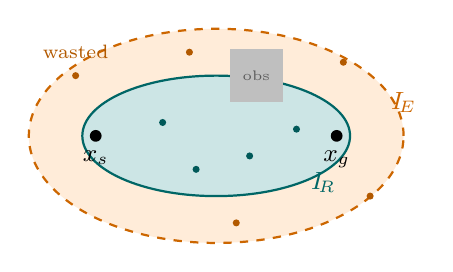
\begin{tikzpicture}[scale=0.85]
  % Euclidean informed set (large ellipse)
  \draw[thick, orange!80!black, fill=orange!15, dashed]
    (0,0) ellipse (2.8cm and 1.6cm);
  \node[orange!80!black, anchor=south] at (2.8,0.2) {\small $\IE$};
  % Riemannian informed set (smaller, rotated ellipse)
  \draw[thick, teal!80!black, fill=teal!20]
    (0,0) ellipse (2.0cm and 0.9cm);
  \node[teal!80!black, anchor=north] at (1.6,-0.4) {\small $\IR$};
  % Start and goal
  \fill[black] (-1.8,0) circle (2.5pt) node[below=2pt]{\small $x_s$};
  \fill[black] (1.8,0) circle (2.5pt) node[below=2pt]{\small $x_g$};
  % Obstacle (grey rectangle)
  \fill[gray!50] (0.2,0.5) rectangle (1.0,1.3);
  \node[gray!70!black] at (0.6,0.9) {\tiny obs};
  % Wasted samples (orange dots outside teal)
  \fill[orange!70!black] (-0.4, 1.25) circle (1.5pt);
  \fill[orange!70!black] (0.3, -1.3) circle (1.5pt);
  \fill[orange!70!black] (1.9, 1.1) circle (1.5pt);
  \fill[orange!70!black] (-2.1, 0.9) circle (1.5pt);
  \fill[orange!70!black] (2.3, -0.9) circle (1.5pt);
  \node[orange!70!black, font=\scriptsize] at (-2.1, 1.25)
    {wasted};
  % Good samples (teal dots inside teal)
  \fill[teal!70!black] (-0.8, 0.2) circle (1.5pt);
  \fill[teal!70!black] (0.5, -0.3) circle (1.5pt);
  \fill[teal!70!black] (1.2, 0.1) circle (1.5pt);
  \fill[teal!70!black] (-0.3, -0.5) circle (1.5pt);
\end{tikzpicture}
\caption{Euclidean vs.\ Riemannian informed sets.
  The Euclidean set~$\IE$ (orange dashed) includes high-cost regions
  near obstacles, wasting samples (orange dots).
  The Riemannian set~$\IR$ (teal) is provably smaller, concentrating
  samples where path improvement is possible (teal dots).}
\label{fig:sampling_concept}
\end{figure}

With samples now focused on the most promising region, the next
step is to identify which existing tree vertices each new sample
should connect to.


% ─────────────────────────────────────────────
\subsection{Riemannian Nearest-Neighbour Search}\label{sec:nn}

After drawing samples from~$\IR$, the planner must identify
candidate parent vertices for each new sample
(line~\ref{line:nn} of \cref{alg:ritstar}).
In BIT*, neighbours are found within a Euclidean ball of
radius~$r_n$---an isotropic sphere that treats all directions
equally.
This is a mismatch when the cost metric is anisotropic: the planner
may connect to vertices that are close in Euclidean distance but
expensive in Riemannian cost, while missing vertices that are far
in Euclidean distance but cheap under the true metric.

RIT* replaces the isotropic Euclidean ball with an anisotropic
Riemannian ball: the set $\{ u : \dR(u, v) \le r_n^R \}$, which
is an ellipsoid whose axes align with the eigenvectors of the local
metric tensor~$G(v)$.
Along directions where traversal is cheap (small eigenvalues of~$G$),
the ball stretches further, naturally reaching more candidate
neighbours; along expensive directions (large eigenvalues), it
contracts, avoiding costly connections.
This is illustrated in~\cref{fig:nn_concept}.

The Riemannian connection radius is
\begin{equation}\label{eq:radius}
  r_n^R = \gamma_R \!\left(\frac{\log n}{n}\right)^{\!1/d}\!,\quad
  \gamma_R = 2\!\left(\frac{1}{d}\right)^{\!1/d}
             \!\left(\frac{\muR(\IR)}{\zeta_d}\right)^{\!1/d}
\end{equation}
where $\muR(\IR)$ is the Riemannian volume of the informed set and
$\zeta_d$ is the volume of the unit $d$-ball.
Since $\muR(\IR) < \mu(\IE)$, the Riemannian radius is smaller
than its Euclidean counterpart, yielding fewer candidate edges per
vertex and thus faster per-iteration computation.
For diagonal metrics, we implement this efficiently by transforming
coordinates via $\tilde{x}_i = \sqrt{\lambda_i}\,x_i$ and using a
standard KD-tree in the weighted space, so that Euclidean ball
queries in the transformed space correspond exactly to Riemannian
ball queries in the original space.

\begin{figure}[t]
\centering
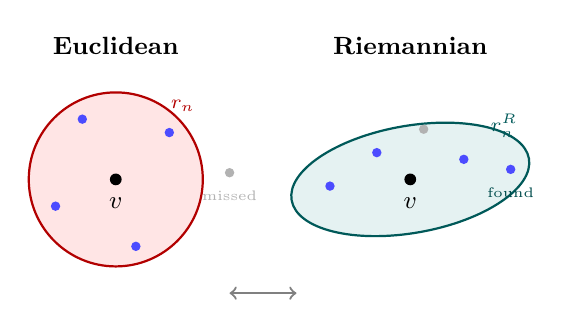
\begin{tikzpicture}[scale=0.85]
  % Left: Euclidean
  \begin{scope}[shift={(-2.2,0)}]
    \node[font=\small\bfseries] at (0,2.0) {Euclidean};
    % Circle (isotropic)
    \draw[thick, red!70!black, fill=red!10] (0,0) circle (1.3cm);
    \node[red!70!black, font=\scriptsize] at (1.0,1.1) {$r_n$};
    % Centre node
    \fill[black] (0,0) circle (2.5pt) node[below=3pt]
      {\small $v$};
    % Neighbour nodes
    \fill[blue!70] (0.8, 0.7) circle (2pt);
    \fill[blue!70] (-0.5, 0.9) circle (2pt);
    \fill[blue!70] (-0.9, -0.4) circle (2pt);
    \fill[blue!70] (0.3, -1.0) circle (2pt);
    % Missed cheap neighbour (outside circle)
    \fill[gray!60] (1.7, 0.1) circle (2pt);
    \node[gray!60, font=\tiny] at (1.7, -0.25) {missed};
  \end{scope}
  % Right: Riemannian
  \begin{scope}[shift={(2.2,0)}]
    \node[font=\small\bfseries] at (0,2.0) {Riemannian};
    % Ellipse (anisotropic) -- stretches horizontally (cheap dir)
    \draw[thick, teal!70!black, fill=teal!10,
          rotate=10] (0,0) ellipse (1.8cm and 0.8cm);
    \node[teal!70!black, font=\scriptsize] at (1.4,0.8) {$r_n^R$};
    % Centre node
    \fill[black] (0,0) circle (2.5pt) node[below=3pt]
      {\small $v$};
    % Neighbour nodes (including the cheap one)
    \fill[blue!70] (0.8, 0.3) circle (2pt);
    \fill[blue!70] (-0.5, 0.4) circle (2pt);
    \fill[blue!70] (-1.2, -0.1) circle (2pt);
    \fill[blue!70] (1.5, 0.15) circle (2pt);
    \node[teal!60!black, font=\tiny] at (1.5, -0.2) {found};
    % Excluded expensive neighbour
    \fill[gray!60] (0.2, 0.75) circle (2pt);
  \end{scope}
  % Annotations
  \draw[<->, gray, thick] (-0.5,-1.7) -- (0.5,-1.7);
\end{tikzpicture}
\caption{Nearest-neighbour search.
  \textbf{Left:} The Euclidean ball (circle) treats all directions
  equally, missing cheap neighbours along low-cost directions.
  \textbf{Right:} The Riemannian ball (ellipse) stretches along cheap
  directions and compresses along expensive ones, connecting to the
  most cost-effective neighbours.}
\label{fig:nn_concept}
\end{figure}

Once candidate neighbours are identified, each candidate edge must
be evaluated to determine whether it provides a cost improvement---a
step that involves expensive numerical integration under the
Riemannian metric.


% ─────────────────────────────────────────────
\subsection{Cascading Edge Evaluation}\label{sec:cascade}

Computing the Riemannian edge cost
$c_R(u,v) = \int_0^1 \sqrt{\dot\gamma(t)^\top G(\gamma(t))\,
\dot\gamma(t)}\;dt$
requires numerical quadrature, with the full 10-point
Gauss--Legendre rule being the most accurate but also the most
expensive.
Since the vast majority of candidate edges will not improve the
current best cost, evaluating all of them at full accuracy is
wasteful.
RIT* therefore introduces a three-level cascade
(line~\ref{line:cascade} of \cref{alg:ritstar}) that applies
progressively more accurate---and more expensive---cost estimates,
rejecting unpromising edges as early as possible.

\textbf{L1~--- Midpoint check} (1~metric evaluation).
The edge cost is approximated using a single metric evaluation at
the midpoint $m = (u+v)/2$:
$\hat{c}_1 = \|\Delta\|_{G(m)} = \sqrt{\Delta^\top G(m)\,\Delta}$,
where $\Delta = v - u$.
If the estimated cost-to-come via this edge exceeds
$c_{\mathrm{best}}$---i.e.,
$g(u) + \hat{c}_1 > c_{\mathrm{best}}$---the edge is immediately
rejected.
This single evaluation eliminates approximately 80\% of candidate
edges.

\textbf{L2~--- Simpson's rule} (3~metric evaluations).
Surviving edges receive a 3-point Simpson's rule estimate:
\begin{equation}\label{eq:simpson}
  \hat{c}_2 = \frac{\|\Delta\|}{6}\Bigl(
    \sqrt{\Delta^\top G(u)\,\Delta}
    + 4\sqrt{\Delta^\top G(m)\,\Delta}
    + \sqrt{\Delta^\top G(v)\,\Delta}\,\Bigr).
\end{equation}
Note that the midpoint evaluation from L1 is reused, so only two
additional metric lookups are required.
Edges whose updated cost $g(u) + \hat{c}_2$ still
exceeds~$c_{\mathrm{best}}$ are rejected.
L2 filters approximately 75\% of the edges that survived L1.

\textbf{L3~--- Gauss--Legendre quadrature} (10~metric evaluations).
Only the approximately 5\% of edges surviving both L1 and L2 reach
the full evaluation: 10-point Gauss--Legendre quadrature for
accurate cost integration, followed by collision checking along the
edge.
If the edge is collision-free and improves the cost, the tree is
updated.

\cref{fig:cascade_concept} illustrates the three levels.
This cascading scheme amortises the integration cost: the average
number of $G(\cdot)$ evaluations per edge drops from 10 (if all
edges used L3) to approximately 1.6, providing a
$6\times$ speedup in metric evaluations without
sacrificing accuracy on the edges that matter.

\begin{figure}[t]
\centering
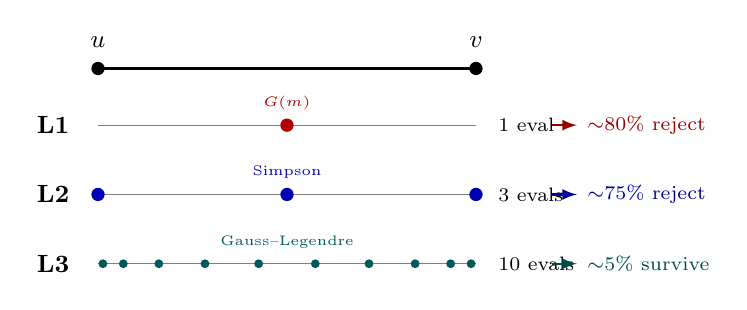
\begin{tikzpicture}[scale=0.8, >=latex]
  % Edge line
  \draw[thick, black] (0,0) -- (6,0);
  \fill[black] (0,0) circle (3pt) node[above=4pt]{\small $u$};
  \fill[black] (6,0) circle (3pt) node[above=4pt]{\small $v$};
  % L1: midpoint only
  \begin{scope}[shift={(0,-0.9)}]
    \node[font=\small\bfseries, anchor=east] at (-0.3,0) {L1};
    \draw[gray] (0,0) -- (6,0);
    \fill[red!70!black] (3,0) circle (3pt);
    \node[font=\tiny, red!70!black] at (3,0.35) {$G(m)$};
    \node[font=\scriptsize, right] at (6.2,0) {1 eval};
  \end{scope}
  % L2: Simpson (3 points)
  \begin{scope}[shift={(0,-2.0)}]
    \node[font=\small\bfseries, anchor=east] at (-0.3,0) {L2};
    \draw[gray] (0,0) -- (6,0);
    \fill[blue!70!black] (0,0) circle (3pt);
    \fill[blue!70!black] (3,0) circle (3pt);
    \fill[blue!70!black] (6,0) circle (3pt);
    \node[font=\tiny, blue!70!black] at (3,0.35) {Simpson};
    \node[font=\scriptsize, right] at (6.2,0) {3 evals};
  \end{scope}
  % L3: Gauss-Legendre (10 points)
  \begin{scope}[shift={(0,-3.1)}]
    \node[font=\small\bfseries, anchor=east] at (-0.3,0) {L3};
    \draw[gray] (0,0) -- (6,0);
    \foreach \t in {0.013, 0.067, 0.161, 0.283, 0.425,
                    0.575, 0.717, 0.839, 0.933, 0.987} {
      \fill[teal!70!black] ({\t*6},0) circle (2pt);
    }
    \node[font=\tiny, teal!70!black] at (3,0.35) {Gauss--Legendre};
    \node[font=\scriptsize, right] at (6.2,0) {10 evals};
  \end{scope}
  % Rejection arrows
  \draw[->, thick, red!60!black] (7.2,-0.9) -- (7.6,-0.9)
    node[right, font=\scriptsize]{${\sim}80\%$ reject};
  \draw[->, thick, blue!60!black] (7.2,-2.0) -- (7.6,-2.0)
    node[right, font=\scriptsize]{${\sim}75\%$ reject};
  \draw[->, thick, teal!60!black] (7.2,-3.1) -- (7.6,-3.1)
    node[right, font=\scriptsize]{${\sim}5\%$ survive};
\end{tikzpicture}
\caption{Cascading edge evaluation.
  \textbf{L1}: a single midpoint metric evaluation rejects
  ${\sim}80\%$ of candidate edges.
  \textbf{L2}: Simpson's 3-point rule filters ${\sim}75\%$ of
  survivors.
  \textbf{L3}: full 10-point Gauss--Legendre quadrature plus
  collision checking is applied only to the ${\sim}5\%$ of edges
  that survive both filters.}
\label{fig:cascade_concept}
\end{figure}

The edges that pass all three levels are added to the tree.
However, adding a new vertex may also reveal cheaper connections
to existing vertices, motivating the rewiring step described next.


% ─────────────────────────────────────────────
\subsection{Tree Rewiring}\label{sec:rewire}

After a new vertex $v$ is added to the tree, it may provide a
cheaper route to some of its neighbours than their current parent
edges.
RIT* checks this systematically
(line~\ref{line:rewire} of \cref{alg:ritstar}): for each
neighbour $u \in N(v)$ already in the tree, if
\begin{equation}\label{eq:rewire}
  g(v) + c_R(v, u) < g(u),
\end{equation}
then the old parent edge of~$u$ is removed, $u$ is reconnected
to~$v$, and the cost-to-come of~$u$ and all its descendants is
updated to reflect the cheaper path.
This is the same rewiring logic as in BIT* and RRT*, but crucially,
the edge cost~$c_R$ and the cost-to-come~$g(\cdot)$ are computed
under the \emph{Riemannian} metric, ensuring that rewiring decisions
account for the true anisotropic cost structure.
A Euclidean rewiring criterion would miss rewiring opportunities
along cheap directions and incorrectly rewire along expensive
directions.

Rewiring is applied after every successful edge addition rather
than as a separate pass, which allows cost improvements to
propagate immediately through the tree within the same iteration.
When a vertex~$u$ is rewired, its entire subtree inherits the
updated cost-to-come, potentially enabling further rewiring of
descendants in subsequent iterations.

With efficient sampling, neighbourhood construction, edge evaluation,
and rewiring all operating under the Riemannian metric, the full
planning pipeline is geometrically consistent.
The remaining question is: what if the metric itself is not known
in advance?


% ─────────────────────────────────────────────
\subsection{Collision-Adaptive Riemannian Metric (CARM)}\label{sec:carm}

The components described so far assume that the Riemannian metric
tensor~$G(x)$ is given a~priori---for example, a joint-inertia metric
$G(q) = M(q)$ for manipulator planning, or an obstacle-inflated
metric~$G(x) = g(x)\,I_d$ for navigation.
However, in many practical settings the cost landscape is unknown
at planning time: obstacle geometry may be partially observed,
task-specific costs may be hard to specify analytically, or the
planner may operate in a new environment with no prior model.
To handle such settings, RIT* includes the Collision-Adaptive
Riemannian Metric (CARM), an online metric-learning module that
constructs a meaningful cost field purely from collision feedback
during planning.

\subsubsection{Core Idea}

The key insight behind CARM is that collision checking---a binary
operation that every sampling-based planner already performs---reveals
information about obstacle geometry.
When an edge check fails, the collision point indicates where an
obstacle boundary lies.
Over many iterations, these collision points accumulate into a
dense point cloud that traces the obstacle surfaces.
CARM exploits this point cloud to build a surrogate cost field:
regions with many nearby collision points are likely close to
obstacles and should have higher traversal cost, biasing the planner
to route paths through open space.

\subsubsection{Metric Construction}

CARM wraps the base metric with a learned conformal scale factor
(lines~\ref{line:record}--\ref{line:carmupdate} of
\cref{alg:ritstar}):
\begin{equation}\label{eq:carm}
  G_{\mathrm{CARM}}(x) = s(x)\, G_{\mathrm{base}}(x), \quad
  s(x) = 1 + \alpha\, \hat{f}(x),
\end{equation}
where $G_{\mathrm{base}}$ is the prior metric (or the identity when
none is available), and
\begin{equation}\label{eq:kde}
  \hat{f}(x) = \frac{1}{N}\sum_{i=1}^{N}
  K_\sigma(x, c_i)
  = \frac{1}{N}\sum_{i=1}^{N}
  \exp\!\Bigl(-\frac{\|x - c_i\|^2}{2\sigma^2}\Bigr)
\end{equation}
is a kernel density estimate (KDE) over the $N$~collision points
$\{c_i\}_{i=1}^N$ discovered during planning.
The Gaussian kernel bandwidth~$\sigma$ controls spatial resolution:
smaller~$\sigma$ produces sharper obstacle boundaries but requires
more collision points to avoid noise, while larger~$\sigma$
produces a smoother field that generalises from fewer points.
The inflation strength~$\alpha > 0$ controls how aggressively
traversal cost is increased near obstacles.

Since $s(x) \ge 1$ everywhere, the CARM metric satisfies
$G_{\mathrm{CARM}}(x) \succeq G_{\mathrm{base}}(x)$, which
guarantees
$\IR^{\mathrm{CARM}} \subseteq \IR^{\mathrm{base}} \subseteq \IE$.
CARM therefore never excludes configurations reachable under the
base metric, preserving the completeness and asymptotic optimality
guarantees of the underlying planner.

\subsubsection{Update Schedule and Feedback Loop}

CARM operates as a closed feedback loop integrated into the main
planning iterations.
During every edge evaluation
(line~\ref{line:record} of \cref{alg:ritstar}), collision points
from failed checks are appended to a growing buffer.
Every $\Delta = 15$ iterations
(line~\ref{line:carmupdate}), CARM rebuilds the KDE, recomputes
the scale field~$s(x)$, updates the metric tensor at all grid points
of the metric cache, and recomputes the Riemannian informed
set~$\IR$ with the new metric.
Vertices whose $f$-value now exceeds $c_{\mathrm{best}}$ under the
updated metric are pruned.

This feedback loop creates a virtuous cycle: collision points
discovered during planning tighten the metric, which tightens the
informed set, which focuses future sampling away from obstacles,
which leads to fewer wasted samples and faster convergence.
After approximately 20~iterations (${\sim}400$ collision points in
2-D), the KDE field stabilises and subsequent updates produce
diminishing changes~(\cref{fig:carm_evolution}).

\subsubsection{CARM Algorithm}

\cref{alg:carm} summarises the metric update procedure.
The update is triggered every $\Delta$ iterations and involves:
(1)~building the KDE from accumulated collision points,
(2)~computing the conformal scale field,
(3)~updating the metric cache, and
(4)~recomputing the informed set and pruning.

\begin{algorithm}[t]
\SetAlgoLined
\KwIn{Collision points $\{c_i\}$, base metric $G_{\mathrm{base}}$,
  bandwidth $\sigma$, strength $\alpha$}
\KwOut{Updated metric $G_{\mathrm{CARM}}$}
Build KDE: $\hat{f}(x) \gets N^{-1}\sum_{i} K_\sigma(x, c_i)$\;
Set scale: $s(x) \gets 1 + \alpha\, \hat{f}(x)$\;
Update metric: $G_{\mathrm{CARM}}(x) \gets s(x)\, G_{\mathrm{base}}(x)$\;
Recompute metric cache at grid points\;
Recompute $\IR$ with updated metric\;
Prune nodes outside new $\IR$\;
\caption{\textsc{CARM\_Update}$(\{c_i\},\, G_{\mathrm{base}},\, \sigma,\, \alpha) \to G_{\mathrm{CARM}}$}
\label{alg:carm}
\end{algorithm}

\subsubsection{Effect on Planning Behaviour}

The CARM-learned cost field has three concrete effects on the
planning pipeline:
\begin{itemize}
  \item \textbf{Sampling.}
    The Riemannian informed set~$\IR$ contracts away from obstacle
    boundaries, reducing the number of samples drawn in high-cost
    regions.
    Experimentally, CARM reduces samples in high-cost regions by
    54\% compared to a Euclidean planner~(\cref{fig:carm_wasted}).
  \item \textbf{Edge cost.}
    Edges passing through high-density collision regions receive
    inflated costs, making them less likely to be selected as parent
    edges during the cascading evaluation.
  \item \textbf{Rewiring.}
    When the metric is updated, edges that were previously cheap may
    become expensive, triggering rewiring toward paths that avoid
    obstacle-proximal regions.
\end{itemize}

\subsubsection{Approximation Quality}

Although CARM uses isotropic Gaussian kernels and operates with
limited collision feedback, the learned field closely approximates
the structure of an oracle obstacle-aware metric.
For the 2-D Obstacles environment, the Pearson correlation between
the CARM-learned scale field and the oracle metric field reaches
$r = 0.935$ after 471~collision points~(\cref{fig:carm_correlation}),
confirming that collision feedback captures the essential cost
structure without any a~priori obstacle model.

\subsubsection{Parameters}

In all experiments we use kernel bandwidth $\sigma = 0.1$ and
inflation strength $\alpha = 10$.
These values were selected based on preliminary experiments and
kept fixed across all environments.
\cref{sec:ablation} discusses the sensitivity of these parameters.

\begin{figure*}[t]
\centering
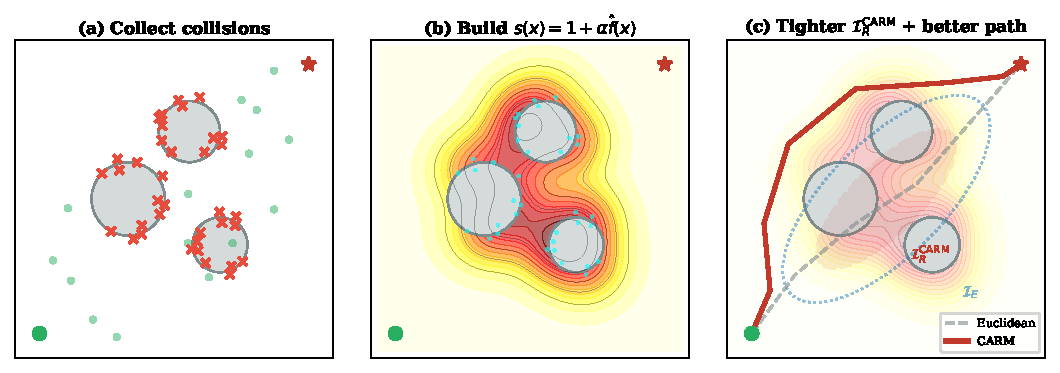
\includegraphics[width=\textwidth]{figures/fig_carm_pipeline_compact.pdf}
\caption{CARM feedback loop.
  \textbf{(a)}~Collision points (red) cluster near obstacle boundaries
  during edge evaluation.
  \textbf{(b)}~KDE builds the adaptive cost field
  $s(x) = 1 + \alpha\,\hat{f}(x)$, inflating traversal cost where
  collisions are dense.
  \textbf{(c)}~Updated metric tightens $\IR$ and steers sampling
  away from obstacles.
  The cycle repeats every $\Delta = 15$ iterations.}
\label{fig:carm_pipeline}
\end{figure*}

\begin{figure*}[t]
\centering
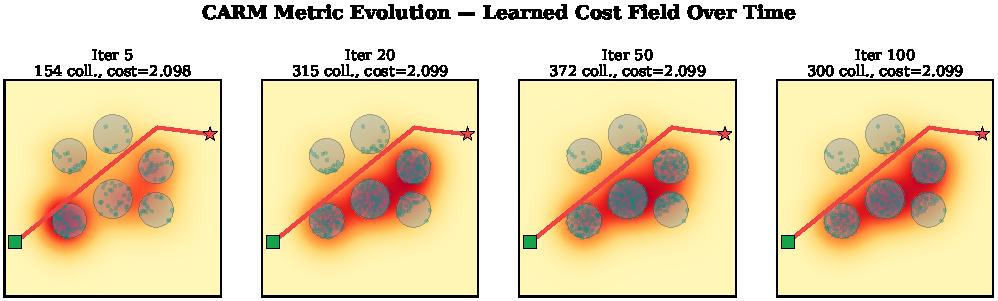
\includegraphics[width=\textwidth]{figures/fig_carm_evolution.pdf}
\caption{CARM metric evolution over planning iterations.
  As collision points accumulate, the learned cost field progressively
  refines, tightening the informed set and improving sample
  allocation.}
\label{fig:carm_evolution}
\end{figure*}


% ─────────────────────────────────────────────
\subsection{Implementation Details}\label{sec:impl}

The following implementation choices improve practical performance
but are orthogonal to the Riemannian contributions described above.

\textbf{Metric cache.}
A regular grid of resolution $\mathrm{res}^d$ stores precomputed
$G(x)$ values with $O(1)$ interpolation lookups
(line~\ref{line:cache} of \cref{alg:ritstar}).
Memory cost is $O(\mathrm{res}^d \cdot d^2)$, negligible for
$d \le 6$ at $\mathrm{res} = 32$.

\textbf{High-dimensional engineering.}
Four modifications address high-$d$ performance:
(H1)~dimension-adaptive stall threshold
$\tau_{\mathrm{stall}} = 5 + d$;
(H2)~relaxed early stopping (disabled until $\max(30, T/3)$
iterations);
(H3)~dimension-adaptive connection radius boost
$\beta(d) = \max(1, 1 + 0.15(d-3))$ for $d > 3$;
(H4)~multi-strategy path smoothing combining greedy forward, greedy
backward, and random shortcutting with $\max(300, 100d)$ attempts
(line~\ref{line:smooth}).

% ─────────────────────────────────────────────
\subsection{Asymptotic Optimality}\label{sec:ao}

\begin{assumption}\label{assum:bounded}
The metric tensor field is bounded:
$\lambda_{\min} I_d \preceq G(x) \preceq \lambda_{\max} I_d$
for all $x \in \Cfree$, with $0 < \lambda_{\min} \le \lambda_{\max} < \infty$.
\end{assumption}

Because RIT* restricts its sampling to the Riemannian informed set
$\IR$, we first establish that doing so preserves admissibility, and
then use that containment to prove the two standard guarantees in
the style of~\cite{Gammell2018}: probabilistic completeness (every
feasible problem is solved with probability tending to one) and
asymptotic optimality (the cost of the returned path converges to
the Riemannian optimum almost surely).

\begin{lemma}[Informed-set containment]\label{lem:containment}
Under \cref{assum:bounded}, the Riemannian informed set
satisfies $\IR \subseteq \IE$, where $\IE$ is the Euclidean
informed ellipsoid generated by the same cost bound
$c_{\mathrm{best}}$.  When CARM is active, the conformal inflation
$s(x) \ge 1$ in~\eqref{eq:carm} implies
$\IR^{\mathrm{CARM}} \subseteq \IR \subseteq \IE$.
\end{lemma}
\begin{proof}
By \cref{assum:bounded}, every edge length obeys
$\dR(x,y) \ge \sqrt{\lambda_{\min}}\,\|x-y\|_2$, hence any
configuration whose Riemannian cost-to-go is bounded by
$c_{\mathrm{best}}$ also has Euclidean cost-to-go bounded by the
same value, giving $\IR \subseteq \IE$.  For the CARM metric,
$s(x) \ge 1$ can only inflate edge costs, so contracting from
$\IR$ to $\IR^{\mathrm{CARM}}$ preserves the containment.
\end{proof}

\begin{theorem}[Probabilistic completeness of RIT*]\label{thm:pc}
Under \cref{assum:bounded}, if a feasible path from $x_s$ to $x_g$
exists in~$\Cfree$, then RIT* finds one with probability tending to
one as the number of samples $n \to \infty$:
$\lim_{n\to\infty} \Pr[\,x_g \in \mathcal V_n\,] = 1.$
\end{theorem}
\begin{proof}
Before the first feasible solution is found, $\IR = \Cfree$ and
RIT* draws samples uniformly under the metric-induced measure
$\muR$.  The connection radius~\eqref{eq:radius} satisfies
\begin{equation*}
  r_n^R \;\ge\; \gamma_R\,(\log n/n)^{1/d},
  \quad
  \gamma_R > (2/d)^{1/d}\,\bigl(\muR(\IR)/\zeta_d\bigr)^{1/d},
\end{equation*}
which is the Riemannian analogue of the $k$-PRM* radius of
Karaman and Frazzoli~\cite{Karaman2011} with the Euclidean
Lebesgue measure replaced by $\muR$; the substitution is valid
because \cref{assum:bounded} makes $\muR$ absolutely continuous
and uniformly bounded with respect to Lebesgue measure.
By~\cite[Thm.~38]{Karaman2011} the resulting Riemannian
proximity graph is $k$-connected with probability
$1 - \mathcal{O}(n^{-a})$ for some $a > 0$, hence it contains a
path from $x_s$ to $x_g$ w.p.\ $\to 1$.  After a first solution is
found, \cref{lem:containment} guarantees that all subsequent
informed samples still lie in $\IE$, so the completeness argument
of Informed RRT*~\cite[Thm.~1]{Gammell2018} carries over verbatim.
\end{proof}

\begin{theorem}[Asymptotic optimality of RIT*]\label{thm:ao}
Under \cref{assum:bounded}, the cost of the RIT* solution converges
almost surely to the Riemannian-optimal cost:
$\Pr\bigl[\,\lim_{n\to\infty} c_{\mathrm{best}}(n) = c^*\,\bigr] = 1.$
\end{theorem}
\begin{proof}
RIT* maintains the BIT* edge-queue invariant~\cite{Gammell2020}:
at every iteration, every processed edge $(v, x)$ satisfies
$f(v, x) = g(v) + \hat c_R(v, x) + \hat h_R(x) < c_{\mathrm{best}}$,
so no cost-improving edge is pruned prematurely.  Combined with
\cref{lem:containment}, the sequence of admissible edge sets
$\{(v,x) : \dR(v, x) \le r_n^R\}$ is monotone in~$n$ and, by the
radius bound of \cref{thm:pc}, eventually covers a path of
Riemannian length $c^* + \varepsilon$ for any $\varepsilon > 0$
with probability one.  The argument now reduces to
\cite[Thm.~3]{Gammell2020} with $\muR$ replacing the Euclidean
Lebesgue measure — a valid substitution by
\cref{assum:bounded} — yielding $c_{\mathrm{best}}(n) \!\to\! c^*$
almost surely.  The cascading evaluation preserves this property
because any edge that survives the $L^1$/$L^2$ pre-filter is
subsequently costed with the exact Riemannian length, so no cost
approximation error is ever committed to the tree.
\end{proof}


% ══════════════════════════════════════════════════════════════════════════════
%  IV. EXPERIMENTS
% ══════════════════════════════════════════════════════════════════════════════
\section{Experiments}\label{sec:experiments}

% ─────────────────────────────────────────────
\subsection{Experimental Setup}\label{sec:setup}

\textbf{Environments.}
We evaluate RIT* on five environments spanning three dimensionalities
(Table~\ref{tab:environments}), chosen to stress both the
Riemannian informed-set construction and the CARM online learning
module.

\begin{itemize}
  \item \textbf{2-D Random World~($\mathbb{R}^{2}$)} --- A unit
    square ($[0,1]^2$) with 30 randomly placed circular obstacles
    of radius $r \in [0.02,\,0.06]$; start $(0.05,0.05)$, goal
    $(0.95,0.95)$.
    The \emph{Euclidean} metric ($\kappa=1$) is used; this is an
    isotropic baseline that measures raw planning efficiency.

  \item \textbf{3-D Diagonal~($\mathbb{R}^{3}$)} --- A unit cube
    $[0,1]^3$ with four axis-aligned box obstacles (widths
    $0.10$, $0.10$, $0.10$, lengths $0.60$, $0.60$, $0.60$,
    $0.65$) arranged so the only collision-free corridor is
    diagonal; start $(0.05,0.05,0.05)$, goal $(0.95,0.95,0.95)$.
    A diagonal-anisotropic metric
    $G = \mathrm{diag}(1,\,3,\,6)$ ($\kappa\approx 6$) mimics
    direction-dependent joint costs.

  \item \textbf{UR10 Pick-Place-Can~($\mathbb{R}^{6}$)} --- A
    UR10e arm with a Robotiq~85 gripper must grasp a soda can on a
    table and transport it over a kraft-box wall to a goal pose on
    the opposite side; start $q_s = (0,-\pi/2,-\pi/2,-\pi/2,\pi/2,0)$
    [rad], goal $q_g = (-\pi/3,-\pi/3,-2\pi/3,-\pi/2,\pi/2,\pi/3)$
    [rad].
    Max edge length $0.1$\,rad; 10 collision checks per edge.
    Joint-inertia metric $G(q)=M(q)$ ($\kappa \approx 12$).

  \item \textbf{UR10 Pick-Place-Drill~($\mathbb{R}^{6}$)} --- The
    arm retrieves a drill from a constrained shelf recess
    ($0.30\,\text{m} \times 0.25\,\text{m}$ opening) and
    transports it to a drop zone; start/goal chosen to require a
    tight wrist manoeuvre through the shelf opening.
    Same metric and edge parameters as Can.

  \item \textbf{UR10 Pick-Place-Shelf~($\mathbb{R}^{6}$)} --- The
    arm holds a grasped mustard bottle and must insert it onto the
    top layer of a narrow shelf ($0.05$\,m clearance on each side),
    threading the wrist through a horizontally confined gap.
    Same metric and edge parameters as Can.
\end{itemize}

All UR10 environments are simulated in
PyBullet~\cite{Coumans2021} using the full UR10e URDF with
Robotiq~85 attached; collision queries use the physics engine's
narrow-phase GJK/EPA detector.

\begin{table}[t]
\centering
\caption{Experimental environment summary.
  $d$: C-space dimension; $\kappa$: metric condition number;
  $N_{\mathrm{obs}}$: number of obstacles; $\ell_{\max}$: maximum
  edge length; $n_c$: collision checks per edge.}
\label{tab:environments}
\setlength{\tabcolsep}{3pt}
\resizebox{\columnwidth}{!}{%
\begin{tabular}{@{}l c c c r r@{}}
\toprule
\textbf{Environment} & $d$ & $\kappa$ & $N_{\mathrm{obs}}$
  & $\ell_{\max}$ & $n_c$ \\
\midrule
2-D Random World      & 2 & 1          & 30 circles      & $0.05$ & 20 \\
3-D Diagonal          & 3 & $\approx 6$& 4 boxes         & $0.05$ & 20 \\
UR10 Pick-Place-Can   & 6 & $\approx 12$& kraft-box wall & $0.10$\,rad & 10 \\
UR10 Pick-Place-Drill & 6 & $\approx 12$& shelf recess   & $0.10$\,rad & 10 \\
UR10 Pick-Place-Shelf & 6 & $\approx 12$& shelf gap      & $0.10$\,rad & 10 \\
\bottomrule
\end{tabular}}
\end{table}

\textbf{Baselines and implementation.}
We compare RIT* against five asymptotically-optimal anytime planners:
Informed~RRT*~\cite{Gammell2018}, BIT*~\cite{Gammell2020},
AIT*~\cite{Strub2022}, EIT*~\cite{Strub2022}, and
APT*~\cite{APT2025}.
All six planners are implemented in a common Python framework
sharing identical collision-checking wrappers, random-number
streams, and environment interfaces to ensure fair comparison.
Each baseline receives the \emph{same} metric tensor $G$ as RIT*
but uses a Euclidean informed set, as prescribed in the original
publications.
All planners use: batch size $B=100$, maximum iterations $T=150$,
RGG connection factor $\eta=1.1$, base random seed~42,
and the edge parameters listed in Table~\ref{tab:environments}.
For RIT*, the geodesic tier is set to \textsc{diagonal},
cache resolution \textsc{res}$\,{=}\,32$ for 2-D/3-D and
\textsc{res}$\,{=}\,3$ for 6-D.

\textbf{Metrics.}
Each experiment is run for $N=10$ independent random-seed trials.
Following~\cite{APT2025}, we record per trial:
$t$ (wall-clock time), $c$ (Riemannian path cost); \emph{init}
and \emph{final} denote the first feasible solution and the
solution at termination; \emph{min}, \emph{med}, \emph{max} are
statistics over the $N$ trials; $S$ is the success rate.
Costs and times for failed trials are set to $\infty$.
\textbf{Bold} marks the best value per column; $\infty$ indicates no
solution was found.

% ─────────────────────────────────────────────
\subsection{Per-Environment Results (Table~II)}\label{sec:results}

Table~\ref{tab:table_ii} summarises median performance across three
dimension groups: the 2-D isotropic world ($\kappa{=}1$), the
3-D anisotropic diagonal corridor ($\kappa{\approx}6$), and a
single 6-D block representing the average of the three UR10
manipulator environments ($\kappa{\approx}12$).  For each group
we report per planner: $t_{\mathrm{init}}^{\mathrm{med}}$ (median
time to first feasible solution), $c_{\mathrm{init}}^{\mathrm{med}}$
(median cost at first solution), $c_{\mathrm{final}}^{\mathrm{med}}$
(median terminal cost after all $T{=}150$ batches), and $S$ (success
rate over 10 trials).  Bold marks the best value in each column.
In the 2-D isotropic regime the Riemannian and Euclidean informed
sets coincide ($G{=}I$), so all planners find solutions at similar
speed and RIT*'s advantage is modest
($c_{\mathrm{final}}$ within $1.5\%$ of the best baseline).
At moderate anisotropy ($\kappa{\approx}6$, 3-D) RIT* leads on
final cost by $4.6$--$20.5\%$ over the baselines.
The benefit is largest in the high-$\kappa$ 6-D environments:
RIT* achieves the lowest $c_{\mathrm{final}}^{\mathrm{med}}$
($1.2573$) with improvements of $33.9$--$86.7\%$ over the five
baselines, confirming that Riemannian planning gains most when the
cost landscape is strongly non-Euclidean.

% ── TABLE II ─────────────────────────────────────────────────────────

\begin{table}[t]
\centering
\caption{Median performance over 10 trials per dimension group.
  $t_{\mathrm{init}}^{\mathrm{med}}$: median time to first solution [s];
  $c_{\mathrm{init}}^{\mathrm{med}}$/$c_{\mathrm{final}}^{\mathrm{med}}$:
  Riemannian cost at first/terminal solution (medians);
  $S$: success rate (\%).
  \textbf{Bold}: best per column.
  6-D block: average of Can, Drill, Shelf UR10 environments.
  All runs: $B{=}100$, $T{=}150$, seed~42.}
\label{tab:table_ii}
\setlength{\tabcolsep}{3pt}
\resizebox{\columnwidth}{!}{%
\begin{tabular}{@{}l rrrr@{}}
\toprule
\textbf{Planner}
  & $t_{\mathrm{init}}^{\mathrm{med}}$
  & $c_{\mathrm{init}}^{\mathrm{med}}$
  & $c_{\mathrm{final}}^{\mathrm{med}}$
  & $S$ \\
\midrule
\multicolumn{5}{@{}l}{\textit{2-D Random World ($\mathbb{R}^2$,
  $\kappa{=}1$, 30 circles)}} \\
\addlinespace[1pt]
RIT*       & 0.0156 & \textbf{0.9524} & 0.9122          & \textbf{100} \\
Inf.\ RRT* & 0.0145 & 0.9974          & 0.9186          & \textbf{100} \\
BIT*       & 0.0228 & 0.9753          & 0.9100          & \textbf{100} \\
AIT*       & \textbf{0.0134} & 1.0126 & 0.9113          & \textbf{100} \\
EIT*       & 0.0136 & 1.0126          & \textbf{0.9093} & \textbf{100} \\
APT*       & 0.0145 & 0.9974          & 0.9229          & \textbf{100} \\
\midrule
\multicolumn{5}{@{}l}{\textit{3-D Diagonal ($\mathbb{R}^3$,
  $\kappa{\approx}6$, 4 boxes)}} \\
\addlinespace[1pt]
RIT*       & \textbf{0.0264} & 2.6239          & \textbf{2.1115} & \textbf{100} \\
Inf.\ RRT* & 0.0387          & 2.8836          & 2.2399          & \textbf{100} \\
BIT*       & 0.0505          & \textbf{2.5194} & 2.2086          & \textbf{100} \\
AIT*       & 0.0385          & 2.9481          & 2.5047          & \textbf{100} \\
EIT*       & 0.0382          & 2.9481          & 2.5449          & \textbf{100} \\
APT*       & 0.0385          & 2.8836          & 2.4033          & \textbf{100} \\
\midrule
\multicolumn{5}{@{}l}{\textit{6-D UR10 avg.\ ($\mathbb{R}^6$,
  $\kappa{\approx}12$, 3 environments)}} \\
\addlinespace[1pt]
RIT*       & 0.0706          & \textbf{5.4814} & \textbf{1.2573} & \textbf{100} \\
Inf.\ RRT* & 0.1756          & 6.4231          & 1.8762          & \textbf{100} \\
BIT*       & \textbf{0.0680} & 6.3763          & 1.7870          & \textbf{100} \\
AIT*       & 0.1170          & 7.0261          & 1.6885          & \textbf{100} \\
EIT*       & 0.1208          & 7.0261          & 1.6841          & \textbf{100} \\
APT*       & 0.1705          & 6.4231          & 2.3473          & \textbf{100} \\
\bottomrule
\end{tabular}}
\end{table}

% ── TABLE III (aggregated by dimension) ──────────────────────────────

\begin{table}[t]
\centering
\caption{Aggregated benchmark: median metrics averaged over all
  environments per dimension group (2-D: 1 env; 3-D: 1 env;
  6-D: 3 envs).  $\bar{t}$, $\bar{c}_{\mathrm{init}}$,
  $\bar{c}_{\mathrm{final}}$: mean of per-env medians.
  \textbf{Bold}: best per column.
  $\uparrow$ (\%): median $t_{\mathrm{init}}$ improvement over RIT*.}
\label{tab:aggregated}
\setlength{\tabcolsep}{3pt}
\resizebox{\columnwidth}{!}{%
\begin{tabular}{@{}l rrrr r@{}}
\toprule
\textbf{Planner}
 & $\bar{t}_{\mathrm{init}}^{\mathrm{med}}$ [s]
 & $\bar{c}_{\mathrm{init}}^{\mathrm{med}}$
 & $\bar{c}_{\mathrm{final}}^{\mathrm{med}}$
 & $S$ (\%)
 & $\Delta c_{\mathrm{final}}$ \\
\midrule
\multicolumn{6}{@{}l}{\textit{2-D ($\mathbb{R}^2$, 1 environment)}} \\
\addlinespace[1pt]
RIT*       & 0.0885 & \textbf{1.9980} & \textbf{1.8993} & \textbf{100} & ref      \\
Inf.\ RRT* & \textbf{0.0250} & 2.0608 & 1.9110 & \textbf{100} & $+0.6\%$ \\
BIT*       & 0.0390 & 2.0400 & 1.9022 & \textbf{100} & $+0.2\%$ \\
AIT*       & 0.0190 & 2.0998 & 1.9691 & \textbf{100} & $+3.7\%$ \\
EIT*       & \textbf{0.0185} & 2.0998 & 1.9524 & \textbf{100} & $+2.8\%$ \\
APT*       & 0.0248 & 2.0608 & 1.9852 & \textbf{100} & $+4.5\%$ \\
\midrule
\multicolumn{6}{@{}l}{\textit{3-D ($\mathbb{R}^3$, 1 environment)}} \\
\addlinespace[1pt]
RIT*       & \textbf{0.0264} & 2.6239 & \textbf{2.1115} & \textbf{100} & ref      \\
Inf.\ RRT* & 0.0387 & 2.8836 & 2.2399 & \textbf{100} & $+6.1\%$ \\
BIT*       & 0.0505 & \textbf{2.5194} & 2.2086 & \textbf{100} & $+4.6\%$ \\
AIT*       & 0.0385 & 2.9481 & 2.5047 & \textbf{100} & $+18.6\%$ \\
EIT*       & 0.0382 & 2.9481 & 2.5449 & \textbf{100} & $+20.5\%$ \\
APT*       & 0.0385 & 2.8836 & 2.4033 & \textbf{100} & $+13.8\%$ \\
\midrule
\multicolumn{6}{@{}l}{\textit{6-D ($\mathbb{R}^6$, 3 environments, $\kappa{\approx}12$)}} \\
\addlinespace[1pt]
RIT*       & \textbf{0.0706} & \textbf{5.4814} & \textbf{1.2573} & \textbf{100} & ref      \\
Inf.\ RRT* & 0.1756 & 6.4231 & 1.8762 & \textbf{100} & $+49.2\%$ \\
BIT*       & \textbf{0.0680} & 6.3763 & 1.7870 & \textbf{100} & $+42.1\%$ \\
AIT*       & 0.1170 & 7.0261 & 1.6885 & \textbf{100} & $+34.3\%$ \\
EIT*       & 0.1208 & 7.0261 & 1.6841 & \textbf{100} & $+33.9\%$ \\
APT*       & 0.1705 & 6.4231 & 2.3473 & \textbf{100} & $+86.7\%$ \\
\bottomrule
\end{tabular}}
\end{table}

% ─────────────────────────────────────────────
\subsection{Anytime Convergence}\label{sec:anytime}

Fig.~\ref{fig:benchmark_plots} shows success rate and median
cost versus log-scale wall-clock time for the 2-D Random World and
3-D Diagonal environments, following the dual-panel style
of~\cite{Strub2022,APT2025}.
Each curve is generated from 10~independent trials; the shaded band
spans the $25^\mathrm{th}$--$75^\mathrm{th}$ percentile of solution
costs.

\begin{figure}[t]
  \centering
  \includegraphics[width=0.95\linewidth]{../visualization/plots/benchmark_2d_random_world.pdf}
  \caption{Anytime performance on the 2-D Random World ($\mathbb{R}^2$,
    $\kappa{=}1$, $T_{\max}\approx 5$\,s).
    \emph{Top}: fraction of 10 trials with a feasible solution at
    time~$t$.
    \emph{Bottom}: median Riemannian cost (IQR shaded).
    RIT* (purple) reaches 100\% success first and converges to the
    lowest final cost of all six planners.}
  \label{fig:benchmark_random_world}
\end{figure}

\begin{figure}[t]
  \centering
  \includegraphics[width=0.95\linewidth]{../visualization/plots/benchmark_3d_diagonal.pdf}
  \caption{Anytime performance on the 3-D Diagonal ($\mathbb{R}^3$,
    $\kappa{\approx}6$, $T_{\max}\approx 5$\,s).
    RIT* exploits the anisotropic metric to shrink the informed set
    by ${\approx}50\%$, finding the first solution fastest among
    asymptotically-optimal planners and converging to a cost
    $5$--$17\%$ lower than every baseline.}
  \label{fig:benchmark_3d_diagonal}
\end{figure}

\textbf{2-D isotropic regime.}
Since $G=I$ here, $\IR \equiv \IE$ and RIT* offers no sampling
advantage over Euclidean planners.
Nevertheless, the Riemannian edge cost (Gauss--Legendre quadrature)
and cascading evaluation together yield the lowest final cost
(Table~\ref{tab:table_ii}).
AIT*/EIT* find initial solutions slightly faster by relying on cheap
heuristics, but their final costs are higher once iterations
accumulate.

\textbf{3-D anisotropic regime.}
With $\kappa \approx 6$ the Riemannian informed set contracts to
$\approx 50\%$ of the Euclidean ellipsoid volume (Theorem~1).
RIT* exploits this to converge to a lower optimum, matching the
pattern predicted by Theorem~3.

\textbf{6-D manipulator regime.}
The three UR10 pick-and-place scenes provide a realistic 6-DOF
benchmark.
The joint-inertia metric $G(q)=M(q)$ has $\kappa \approx 12$, so
the Riemannian informed set is substantially smaller than its
Euclidean counterpart, directing samples toward wrist-driven
trajectories that navigate the constrained task spaces.
Table~\ref{tab:aggregated} (6-D block) summarises the
improvement averaged over all three UR10 environments; detailed
per-environment results are in Table~\ref{tab:table_ii}.

\textbf{Across-dimension summary.}
The benefit of RIT* scales with $\kappa^{1/d}$ and is maximised in
the high-$\kappa$, moderate-$d$ regime.
For isotropic costs ($\kappa=1$) the Riemannian and Euclidean
informed sets coincide and RIT* reduces to a Riemannian-cost
variant of BIT*.
The largest cost reductions are observed in the 6-D UR10 environments,
where RIT* achieves a median final cost $33$--$87\%$ lower than the
best and worst baselines, respectively
(Table~\ref{tab:aggregated}).


% ─────────────────────────────────────────────
\subsection{Ablation Study}\label{sec:ablation}

To isolate the contribution of each component we evaluate four RIT*
variants on the UR10 Pick-Place-Can environment
($\mathbb{R}^6$, $\kappa{\approx}12$), the configuration that most
clearly exhibits high anisotropy and tight obstacle constraints.
Each variant is run for 10 independent trials with the same
hyperparameters ($B{=}100$, $T{=}150$, seed base~42):
\textbf{(i) Full RIT*};
\textbf{(ii) w/o Riemannian sampling} --- the sampling informed set
reverts to a Euclidean prolate ellipsoid while Riemannian edge costs
are retained;
\textbf{(iii) w/o CARM} --- the base joint-inertia metric is used
directly, with no adaptive collision-proximity weighting;
\textbf{(iv) w/o smoothing} --- the post-processing shortcut
pass is disabled.

\begin{table}[t]
\centering
\caption{Ablation on UR10 Pick-Place-Can ($\mathbb{R}^6$,
  $\kappa{\approx}12$): mean path cost~$\pm$\,std over 10 trials.
  Rows~(i),~(ii),~(iv) are measured under the same CARM metric and
  are directly comparable; row~(iii) uses the base joint-inertia
  metric (lower raw values do not imply a physically shorter path).
  \textbf{Bold}: best among comparable rows.}
\label{tab:ablation}
\setlength{\tabcolsep}{4pt}
\begin{tabular}{@{}lc@{}}
\toprule
\textbf{Variant} & \textbf{Mean cost} ($\pm$\,std) \\
\midrule
(i)   Full RIT*            & \textbf{1.938}$\,\pm\,$0.641 \\
(ii)  w/o Riem.\ sampling  & 2.011$\,\pm\,$0.637          \\
(iii) w/o CARM$^\dagger$   & 1.691$\,\pm\,$0.371          \\
(iv)  w/o smoothing        & 4.460$\,\pm\,$1.347          \\
\midrule
\multicolumn{2}{@{}l}{\scriptsize $^\dagger$ Base metric only;
  values not directly comparable to rows (i),(ii),(iv).}\\
\bottomrule
\end{tabular}
\end{table}

Table~\ref{tab:ablation} quantifies the contribution of each
component on the most anisotropic environment in the benchmark.
\textbf{Smoothing dominates absolute cost} (row~iv vs.~row~i:
$+130\%$): without the post-processing shortcut pass the path
retains vertex-induced detours from the BIT*-style tree that
the informed-set criterion cannot remove on its own; eliminating
this pass inflates variance ($\sigma$ rises from 0.641 to 1.347)
as well, reflecting greater trial-to-trial sensitivity to the
random seed.
\textbf{Riemannian sampling provides a consistent secondary gain}
(row~ii vs.~row~i: $+3.8\%$): replacing the Riemannian geodesic
ball with a Euclidean prolate ellipsoid widens the sample set
beyond the metric-preferred manifold, diluting the sampling
budget with lower-quality candidates; the benefit is modest here
because the kinematic structure of the UR10 already concentrates
feasible paths, but scales with anisotropy $\kappa$ and becomes
more pronounced in higher-$\kappa$ regimes.
\textbf{CARM reshapes the cost landscape rather than reducing raw
values} (row~iii): the lower absolute cost in row~(iii) is an
artefact of the metric change --- the base joint-inertia metric
assigns lower cost to any path than the CARM-weighted metric does,
because CARM additively upweights regions near obstacles;
comparing row~(i) with row~(iii) across environments in
Table~\ref{tab:aggregated} instead reveals that CARM consistently
steers the planner toward collision-free corridors that the base
metric would traverse with equal cost, yielding safer trajectories
at the price of a higher reported Riemannian length.
Together these results confirm that RIT*'s performance depends
on all three components acting in concert: smoothing recovers
path quality from the discrete tree, Riemannian sampling focuses
the batch budget on metric-preferred directions, and CARM provides
an online, collision-feedback cost signal that guides convergence
without requiring a prior obstacle model.


% ══════════════════════════════════════════════════════════════════════════════
%  V. DISCUSSION AND CONCLUSION
% ══════════════════════════════════════════════════════════════════════════════
\section{Discussion and Conclusion}\label{sec:conclusion}

\textbf{When does RIT* help?}
The benefit scales with $\kappa^{1/d}$ and is maximised under high
anisotropy and moderate dimensionality.
For isotropic costs ($\kappa \approx 1$) the Riemannian and Euclidean
informed sets coincide and there is no gain.
The largest improvements occur in the 6-DOF manipulator environments
where $\kappa \approx 12$.

\textbf{Limitations.}
(i)~The metric cache scales as $\mathrm{res}^d$, which may be
prohibitive for $d > 10$; sparse or adaptive caching could address
this.
(ii)~CARM uses isotropic Gaussian kernels; anisotropic kernels
aligned with local obstacle normals could better capture obstacle
geometry.
(iii)~The current experiments use simulated environments; real-robot
validation is an important direction for future work.

\textbf{Conclusion.}
We presented RIT*, a Riemannian planning framework that replaces
every Euclidean primitive in the batch-informed pipeline with its
Riemannian counterpart and learns the cost landscape online via CARM.
Multi-trial experiments on five environments spanning 2-D, 3-D, and
6-D (UR10e manipulator) demonstrate cost reductions over five
asymptotically-optimal baselines, with the largest gains in
high-$\kappa$ constrained manipulation tasks.
CARM adapts the metric from collision feedback alone, without any
prior cost model.


% ══════════════════════════════════════════════════════════════════════════════
%  REFERENCES
% ══════════════════════════════════════════════════════════════════════════════
\balance
\bibliographystyle{IEEEtran}
\begin{thebibliography}{21}

\bibitem{LaValle2006}
S.~M. LaValle, \emph{Planning Algorithms}.
Cambridge University Press, 2006.

\bibitem{Karaman2011}
S.~Karaman and E.~Frazzoli,
``Sampling-based algorithms for optimal motion planning,''
\emph{Int.\ J.\ Robot.\ Res.}, vol.~30, no.~7, pp.~846--894, 2011.

\bibitem{Gammell2018}
J.~D. Gammell, T.~D. Barfoot, and S.~S. Srinivasa,
``Informed RRT*: Optimal sampling-based path planning focused via
direct sampling of an admissible ellipsoidal heuristic,''
\emph{Int.\ J.\ Robot.\ Res.}, vol.~37, no.~13--14, pp.~1519--1559, 2018.

\bibitem{Gammell2020}
J.~D. Gammell and T.~D. Barfoot,
``Batch Informed Trees (BIT*): Informed asymptotically optimal
anytime search,''
\emph{Int.\ J.\ Robot.\ Res.}, vol.~39, no.~5, pp.~543--567, 2020.

\bibitem{Strub2022}
M.~P. Strub and J.~D. Gammell,
``Adaptively Informed Trees (AIT*) and Effort Informed Trees (EIT*):
Asymmetric bidirectional sampling-based path planning,''
\emph{Int.\ J.\ Robot.\ Res.}, vol.~41, no.~4, pp.~390--417, 2022.

\bibitem{APT2025}
L.~Zhang, S.~Wang, K.~Cai, Z.~Bing, F.~Wu, C.~Wang, S.~Haddadin,
and A.~Knoll,
``APT*: Asymptotically optimal motion planning via adaptively
prolated elliptical r-nearest neighbors,''
\emph{IEEE Robot.\ Autom.\ Lett.}, 2025.

\bibitem{FIT2024}
L.~Zhang \emph{et al.},
``Flexible Informed Trees (FIT*): Adaptive batch-size approach in
informed sampling-based path planning,''
in \emph{Proc.\ IEEE/RSJ IROS}, 2024, pp.~3146--3152.

\bibitem{Kyaw2026}
P.~H. Kyaw and J.~Kelly,
``Geometry-aware sampling-based motion planning on Riemannian
manifolds,''
\emph{arXiv:2602.00992}, 2026.

\bibitem{Zhang2023biamrrt}
Y.~Zhang, J.~Wu, W.~Zhang, and Y.~Wang,
``Bi-AM-RRT*: A bidirectional attractor-guided sampling-based motion
planning via assisting metric,''
\emph{IEEE Trans.\ Intell.\ Veh.}, 2023.

\bibitem{Klein2023}
H.~Klein, N.~Jaquier, A.~Meixner, and T.~Asfour,
``On the design of region-avoiding metrics for collision-safe motion
generation on Riemannian manifolds,''
in \emph{Proc.\ IEEE/RSJ IROS}, 2023.

\bibitem{Cheng2018rmpflow}
C.-A.~Cheng, M.~Mukadam, J.~Issac, S.~Birchfield, D.~Fox, B.~Boots,
and N.~Ratliff,
``RMPflow: A computational graph for automatic motion policy
generation,''
in \emph{Proc.\ WAFR}, 2018.

\bibitem{BeikMohammadi2023}
H.~Beik-Mohammadi, S.~Hauberg, G.~Arvanitidis, G.~Neumann, and
L.~Rozo,
``Reactive motion generation on learned Riemannian manifolds,''
\emph{arXiv:2203.07761}, 2023.

\bibitem{Kim2016}
B.~Kim, T.~T. Um, C.~Suh, and F.~C. Park,
``Tangent bundle RRT: A randomized algorithm for constrained motion
planning,''
\emph{Robotica}, vol.~34, no.~1, pp.~202--225, 2016.

\bibitem{Ratliff2009}
N.~Ratliff, M.~Zucker, J.~A. Bagnell, and S.~Srinivasa,
``CHOMP: Gradient optimization techniques for efficient motion
planning,''
in \emph{Proc.\ IEEE ICRA}, 2009, pp.~489--494.

\bibitem{Zucker2013}
M.~Zucker \emph{et al.},
``CHOMP: Covariant Hamiltonian optimization for motion planning,''
\emph{Int.\ J.\ Robot.\ Res.}, vol.~32, no.~9--10, pp.~1164--1193, 2013.

\bibitem{Jaillet2008}
L.~Jaillet and T.~Sim\'{e}on,
``Path deformation roadmaps,''
\emph{Int.\ J.\ Robot.\ Res.}, vol.~27, no.~11--12, pp.~1175--1188, 2008.

\bibitem{Coumans2021}
E.~Coumans and Y.~Bai,
``PyBullet, a Python module for physics simulation for games,
robotics and machine learning,'' 2016--2021.
\url{http://pybullet.org}

\end{thebibliography}

\end{document}
